\chapter{Sprint2:Configuration de la Pipline.}
\newpage
\textbf{\huge Introduction} \\[1cm]
\textsf{\fontfamily{qtm}\selectfont\scalefont{1.3}
Après avoir vue la configuration de l'architecture cloud aws nous présentent la deuxième sprint, nous commençons par l'objectif de sprint puis l'architecture globale ensuite nous détaillons le diagramme d'utilisation et séquence détaille, Finalement, nous allons exposer la partie réalisation.}


\section{\LARGE Objectif du Sprint}
\textsf{\fontfamily{qtm}\selectfont\scalefont{1.3}Ce sprint est à propos de configurer pipline  dont le but est d'améliorer l'efficacité et la qualité du développement logiciel, tout en minimisant les erreurs et les temps d'arrêt.}

\section{\LARGE Architecture Détaillée}
\textsf{\fontfamily{qtm}\selectfont\scalefont{1.3}Dans cette partie nous allons présenter l'architecture détaillée correspond au sprint.}

\subsection{\Large Diagramme Cas d'utilisation Détaillée}
\textsf{\fontfamily{qtm}\selectfont\scalefont{1.3}Pour éliminer toute ambiguïté et éclaircir le cas d'utilisation, nous présentons le cas en détail.}

\begin{figure}[H]
    \begin{center}
    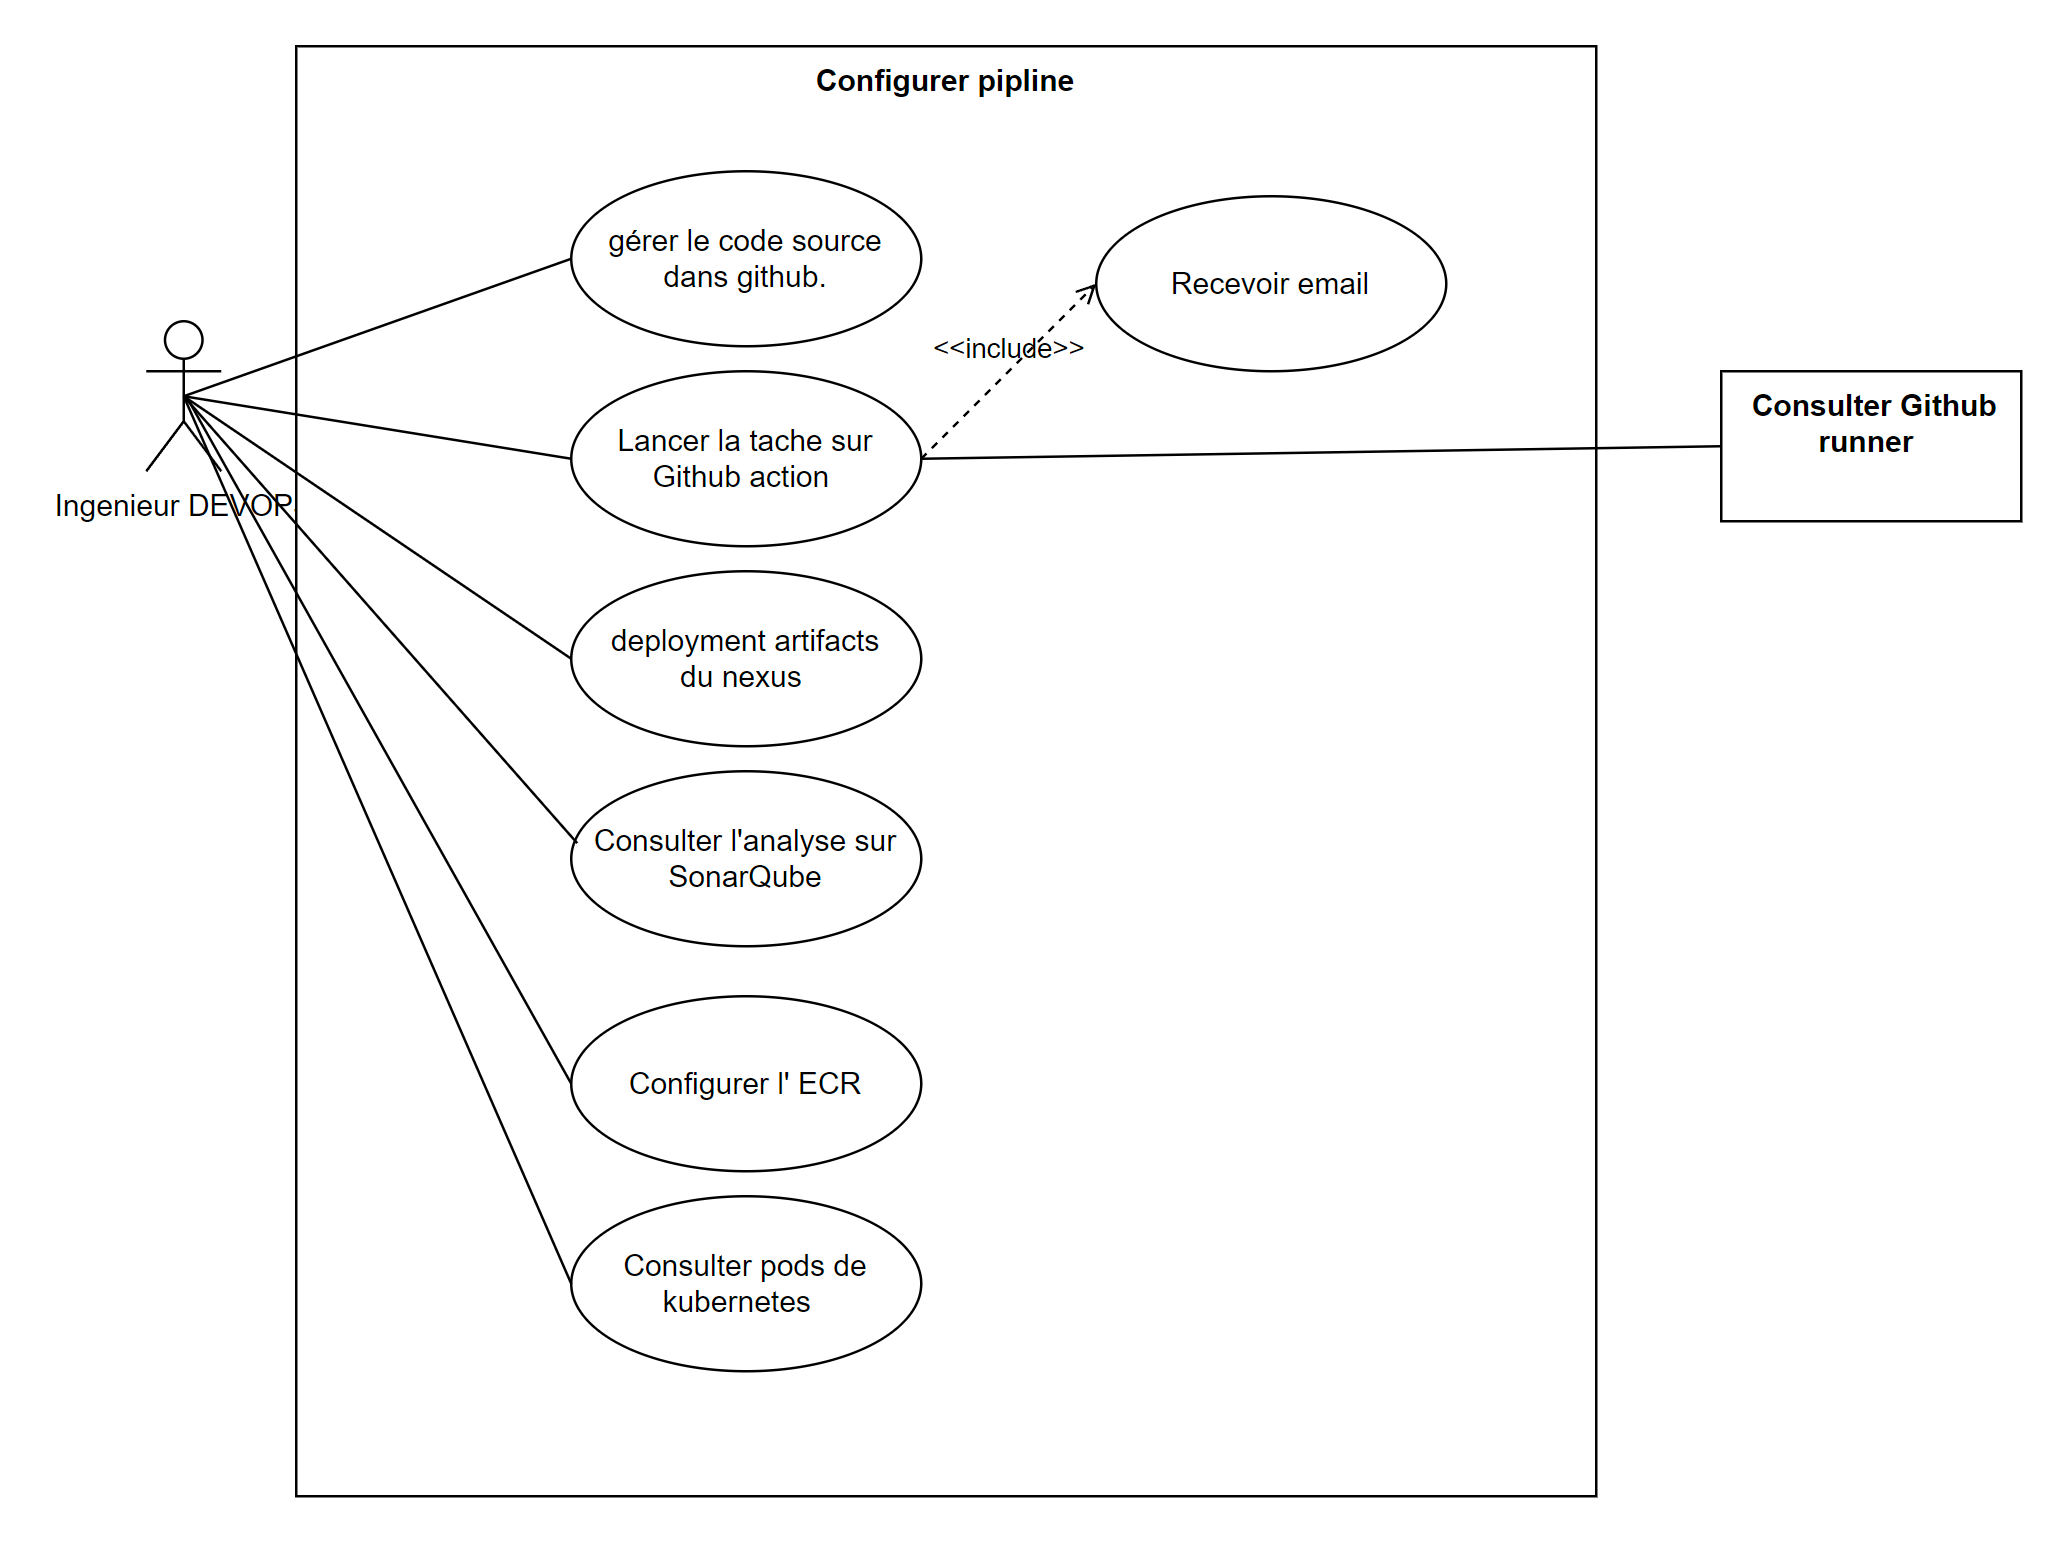
\includegraphics[height=10cm]{configuration pipline use case.png}
    \end{center}
    \caption{cas d’utilisation"Configuration de la Pipline"}
    %\floatfoot{Source: (Citation command)}
    % avec le package "floatrow"
    \end{figure}

\textsf{\fontfamily{qtm}\selectfont\scalefont{1.3}
    Pour expliquer  le diagramme de cas d’utilisation, nous représentons la description textuelle du principales fonctionnalités mentionnées ci-dessus : \\}
    \begin{center}
       \begin{table}[H]  
         \centering
         \resizebox{1.1\textwidth}{!}{%
         \begin{tabular}{|c|p{13cm}|}
          \hline
          Titre & Configuration de la Pipline\\
          \hline
          Acteur & Ingénieur DevOps \\
          \hline
          Description & L'ingénieur DevOps gérait la configuration de la Pipline  et la création du cluster .\\
          \hline
          Pré conditions & Comprendre le processus de déploiement de l' application,
aussi disposer d'une infrastructure appropriée pour prendre en charge le déploiement ,
ainsi identifier les étapes du processus de déploiement, les dépendances et les outils nécessaires.
et pour  automatiser les étapes du pipeline en utilisant des scripts et des configurations. \\
          \hline
          Post conditions & une architecture configurait correctement.  \\
          \hline 
          Scénario nominal & Déploiement continu est réussite et la configuration réussite.\\
          \hline
          Scénario alternatif & problème de compatibilité avec l'infrastructure existante ou la configuration n'est pas correcte.  \\
          \hline
          \end{tabular}%
         }
       \caption{Description de cas d’utilisation}
       \end{table}
       \end{center}
       \subsection{\Large Diagramme de sequance  Détaillée}
       \textsf{\fontfamily{qtm}\selectfont\scalefont{1.3}
       Nous détaillons ci-dessous les interactions générales du système}
       \begin{figure}[H]
    \begin{center}
    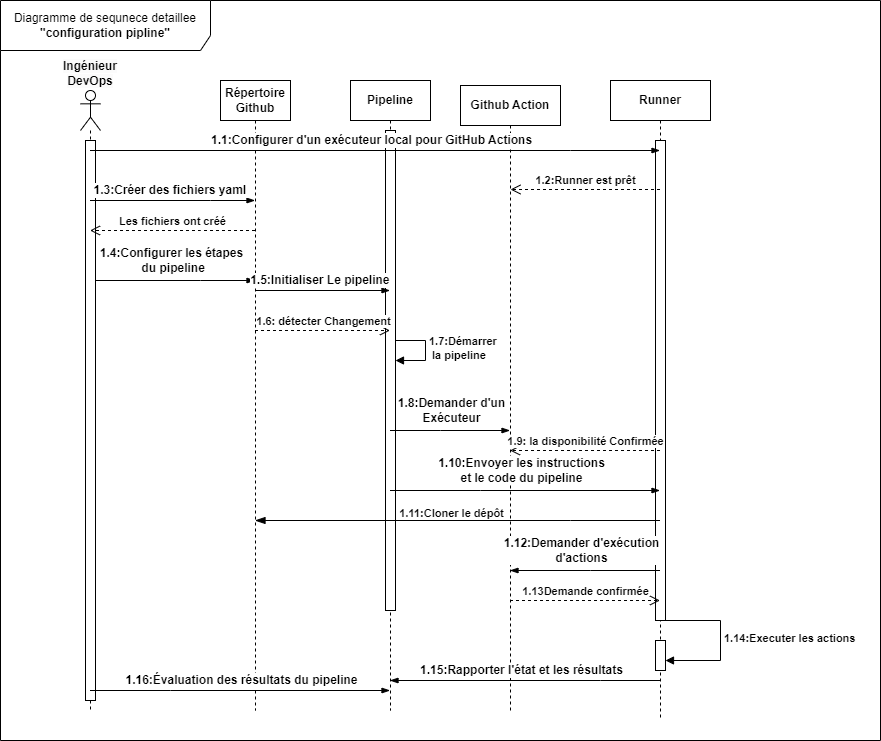
\includegraphics[height=14cm,width=18cm]{sequencepipeline.drawio}
    \end{center}
    \caption{diagramme de séqunce"Configuration de la Pipline"}
    %\floatfoot{Source: (Citation command)}
    % avec le package "floatrow"
    \end{figure}